% !TeX spellcheck = en_US
\addscenariosection{1}{Clash Scenario}{Dragon Valley}{\images/slayer.png}

\begin{multicols*}{2}

\textbf{Author:} LAAMAKALA

\textbf{Source:} \href{https://discord.com/channels/740870068178649108/1239631918643941509}{Archon Studios Discord}

%\textit{A valley where ancient dragons protect secrets long forgotten. Fight for power, claim the land, or perish like those before you.}

\textit{A valley of secrets long forgotten. Its heart belongs to the beasts of old, while its fringes lure the bold and the desperate. Fight for power, claim the land, or perish like those before you.}

% \textit{The valley calls to those who seek adventure and riches beyond imagination. Its heart is guarded by Dragons older than time, its edges lined with settlements of those who dare to claim a foothold in this perilous land. But there is no safety here—only the promise of power for those who fight, and the certainty of death for those who falter.}

\subsection*{\MakeUppercase{Scenario Length}}
This Scenario plays out over 13 Rounds 
%(or a shorter version over 8 Rounds).

\subsection*{\MakeUppercase{Player Setup}}
\textbf{Player Count:} 2 -- 4

\textbf{Starting Resources:} 15 \svg{gold}, 4 \svg{building_materials}, 2 \svg{valuables}

\textbf{Starting Income:} 10 \svg{gold}, 0 \svg{building_materials}, 0 \svg{valuables}

\textbf{Starting Units:}
\begin{itemize}
  \item A Few of \svgunit{bronze} Units of the player's choice
  \item A Pack of \svgunit{bronze} Units of the player's choice
\end{itemize}

\textbf{Town Buildings:}
\begin{itemize}
  \item \svgunit{bronze} Dwelling
  \item Each player may build the \textit{Mage Guild} or a \textit{Faction-specific} building with a discount of 10 \svg{gold} (trading post conversion chart may be used for the discount).
\end{itemize}

\subsection*{\MakeUppercase{Map Setup}}
Take the following Map Tiles and arrange them as shown in the Scenario map layout ($P$ stands for the number of players):

\begin{itemize}
  \item P × Starting (I) Map Tile
  \item 3P × Far (II-III) Map Tiles - one per player must include a Settlement, and one per player must include a Trading Post
  \item 2P × Near (IV-V) Map Tile
  \item P × Center (VI-VII) Map Tiles (C5 is treated as a Settlement)
\end{itemize}

\textbf{Additionally, for 2--3 players:}
\begin{itemize}
  \item 1 × Center (VI-VII) Map Tile with a Dragon Utopia
\end{itemize}

\textbf{For 4 players:}
\begin{itemize}
  \item 2 × Center (VI-VII) Map Tiles with a Dragon Utopia
\end{itemize}

\subsection*{\MakeUppercase{Victory Conditions}}
The game ends at the end of the Round when any of these conditions are met:

\begin{itemize}
 \item One player has defeated all other players' Main Heroes once - \textit{That player wins the game immediately.}
 \item One player conquers both Dragon Utopias - \textit{That player wins the game immediately.}
 \item At the end of Round 13 (or Round 8 for the shorter game).
\end{itemize}

\subsection*{\MakeUppercase{Victory Points}}
If no player has achieved an immediate victory, the player with the most Victory Points (VP) wins:

\begin{itemize}
 \item 5 VP for conquering a Dragon Utopia
 \item 4 VP for controlling 5 Mines or Settlements on Near and Center Tiles - \textit{once per game}
 \item 4 VP for defeating an enemy's Main Hero - \textit{once per defeated Faction}
 \item 2 VP for defeating an enemy's Secondary Hero - \textit{once per defeated Faction}
 \item 2 VP for each enemy Main Town captured - \textit{once per captured Faction}
 \item 1 VP for every controlled Mine or Settlement
% \item 1 VP for every Level of Experience of your Main Hero
\end{itemize}

\subsection*{\MakeUppercase{Timed Events}}

\begin{itemize}
  \item Start of \textbf{\nth{1} Round:} All Heroes gain +1 \svgeven{movement}.
  \item Start of \textbf{\nth{4} Round:} Remove black Cubes from all locations that give resources, morale or Cards (not from Grail).
  \item Start of \textbf{\nth{8} Round:} Repeat event of Round 4.
  \item Start of \textbf{\nth{9} Round:} Repeat event of Round 1.
  \item End of \textbf{\nth{10} Round:} Player(s) with lowest XP roll 2 \svg{resource} dice.
\end{itemize}

\subsection*{\MakeUppercase{Additional Rules}}
\begin{itemize}
  \item Remove ``View Earth'' from the Spell Deck.
  \item Remove ``Unexpected Reinforcements'' from the Astrologers Proclaim Deck.
  \item Create separate Decks for Minor, Major, and Relic Artifacts.
  \item Create separate Decks for Basic and Expert Spells.
  \item On Starting and Far Map Tiles, players can only acquire basic Spells and Minor Artifacts.
  \item Players may not use Diplomacy to skip Level VII Combat.
  \item If your Hero is Level VII, treat Level VI neutrals as Level VII, and gain 10 \svg{gold} for winning a Level VII Combat.
  \item Sanctuary effect: \textbf{once per Faction} gain a \svg{morale_positive}} token and draw 1 Card.
  \item Obelisk effect: \textbf{once per Faction} roll one \svg{resource} and draw one Card.
  \item When fighting a Neutral Combat, a player may add +1 difficulty for an extra 5 \svg{gold} + Search (2) the Artifact or the Spell Deck.
  \item Settlements on Center (VI-VII) Map Tiles are treated as two Settlements in terms of rewards AND allow rolling one \svg{resource} or \svg{treasure} (reroll any XP).
  \item Upon flagging a Grail Field, \textbf{choose one} and then put a Black Cube:
  \begin{itemize}
    \item Receive: 10 \svg{gold}, 4 \svg{building_materials}, and 2 \svg{valuables}.
    \item Roll 2 \svg{treasure} (reroll any XP) and 2 \svg{resource}.
  \end{itemize}
  \item When visiting a Dragon Utopia: Reshuffle the \svgunit{golden} and \svgunit{azure} Decks, then draw from \svgunit{azure} until you get 3 Dragons and choose 2, AND draw from \svgunit{golden} until you get one Dragon.
  \item Upon flagging Dragon Utopia, \textbf{choose one} and then put a Black Cube:
  \begin{itemize}
    \item Recruit one of the defeated Dragons for half its \svg{gold} (rounded down) and its \svg{valuables} cost.
    \item Receive 15 \svg{gold} AND Search (3) any Artifact Deck.
  \end{itemize}
\end{itemize}

After visiting a Dragon Utopia, roll an Attack Die:
\begin{itemize}
  \item[\textbf{-1}] -- Dragons' Curse: The defeated Dragons’ spirits curse the land! All players lose 1 \svgeven{movement} for the next Round.
  \item[\textbf{0}] -- Dragons' Revenge: All players must sacrifice a Unit before the end of the Round; that Unit's health is reduced to 0. 
  \item[ \textbf{+1}] -- Scattered Treasure: All players may immediately spend \mbox{1 \svgeven{movement}} to Search (2) the Artifact Deck.
\end{itemize}

\subsection*{\MakeUppercase{Suggested Houserules}}
\begin{itemize}
  \item Trading Posts - on a single visit, trade Resources and remove Cards, OR buy a War Machines.
%  \item Fighting Neutral Units entails the following:
%  \begin{itemize}
%    \item No Combat Round limit
%    \item On Hard+ difficulty, increase the difficulty of I-IV encounters by one
%    \item Gain Field Level × \svg{gold} as an additional reward
%  \end{itemize}
  \item \href{https://boardgamegeek.com/thread/3445901/custom-hex-combat-board}{Medium Hex combat board}.
  \item \href{https://boardgamegeek.com/thread/3449937/houserule-for-stacking-more-than-pack}{Stacking more than Pack} - Start with Several \svgunit{bronze} Units instead of Few.
\end{itemize}

\vspace*{\fill}

\end{multicols*}

\begin{tikzpicture}[overlay]
  \centering
  % 2-player
  \node at (4.5, -5) {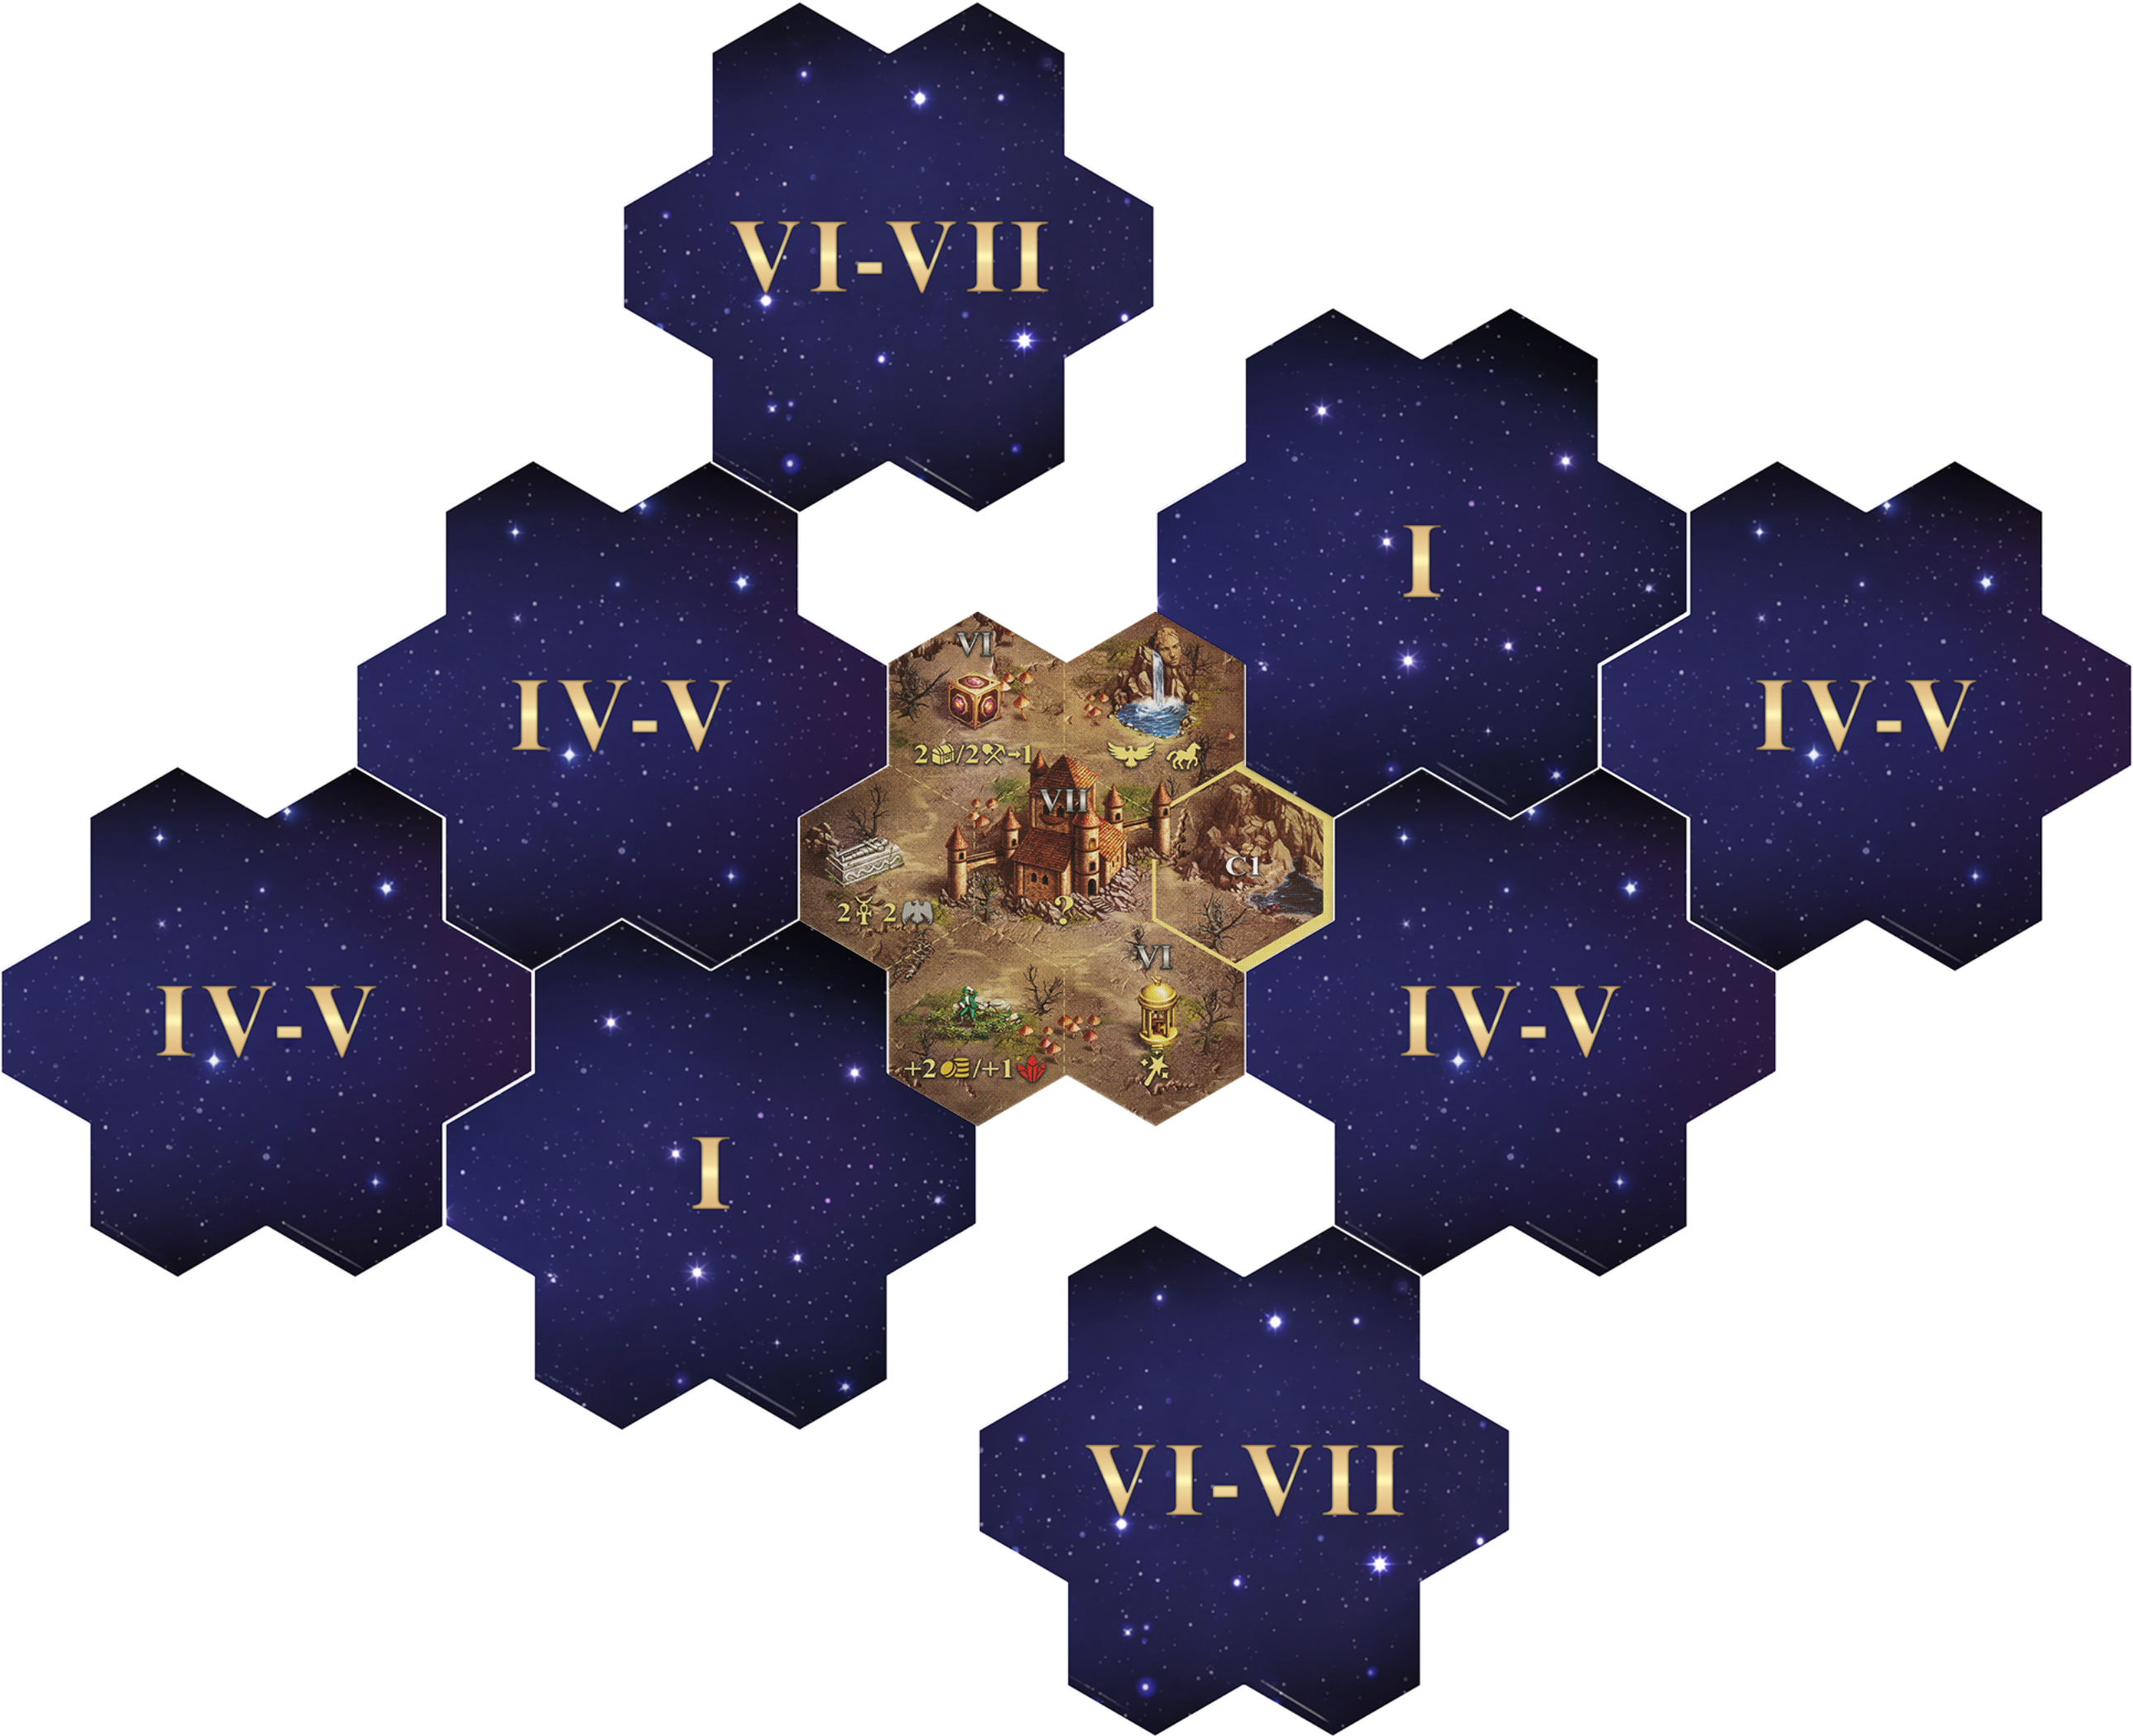
\includegraphics[scale=0.165]{\maps/dragon-valley-2p.png}};
  \node at (4.5, -10) {\footnotesize{\textbf{\MakeUppercase{2-PLAYER SCENARIO}}}};
  % 3-player
  \node at (12.1, -5) {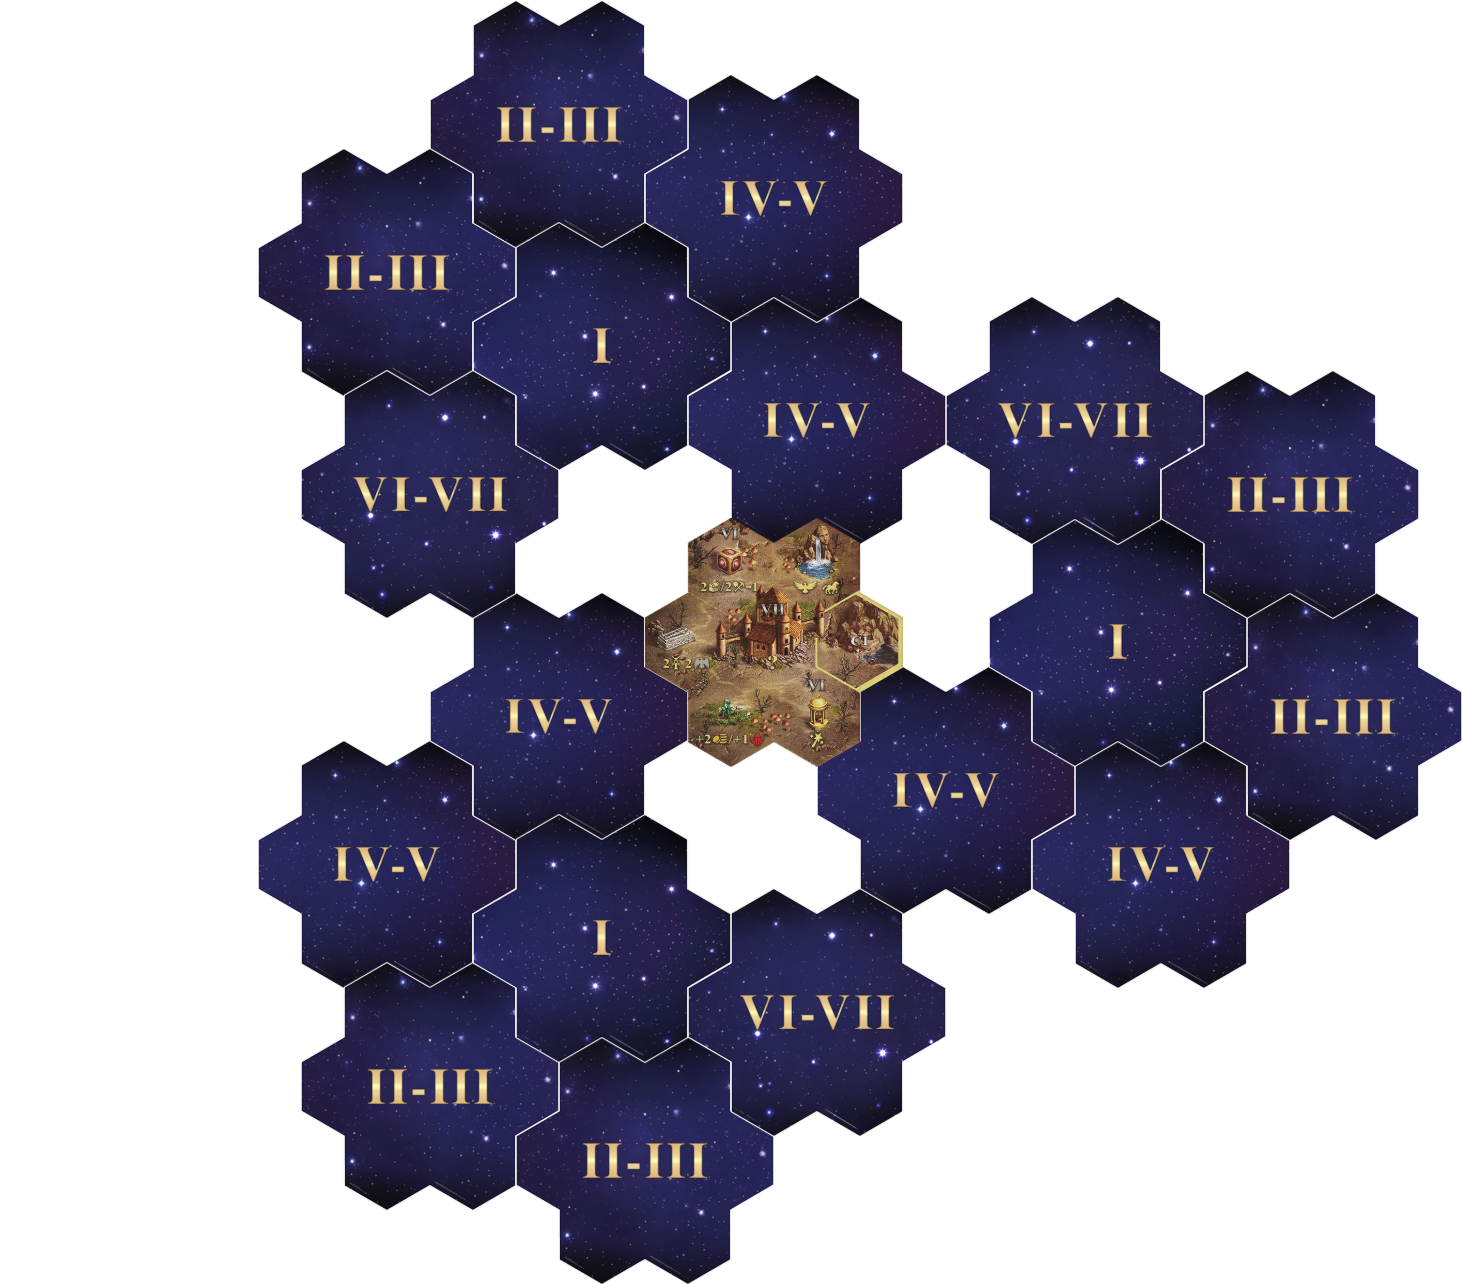
\includegraphics[scale=0.165]{\maps/dragon-valley-3p.png}};
  \node at (12.1, -10) {\footnotesize{\textbf{\MakeUppercase{3-PLAYER SCENARIO}}}};
  % 4-player
  \node at (4.5, -15) {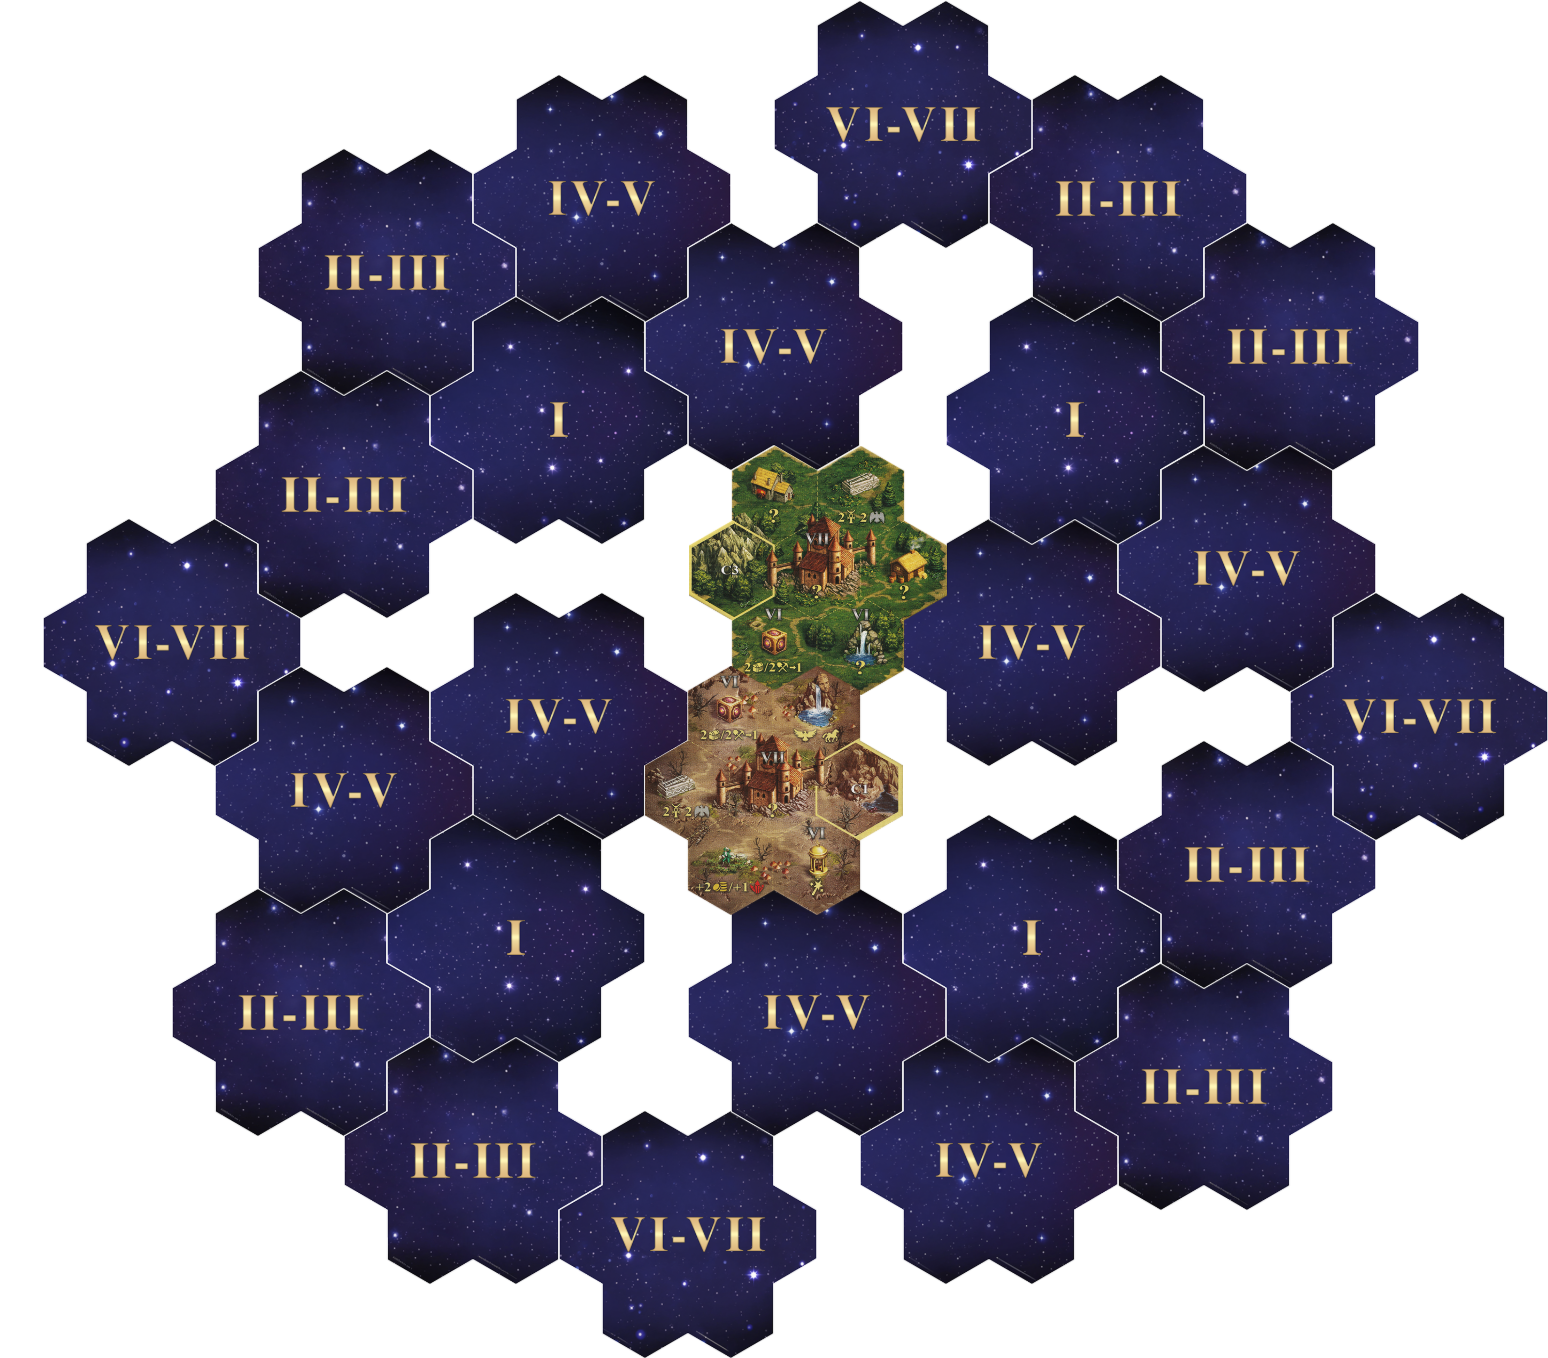
\includegraphics[scale=0.165]{\maps/dragon-valley-4p.png}};
  \node at (4.5, -20) {\footnotesize{\textbf{\MakeUppercase{4-PLAYER SCENARIO}}}};
  % 4-player short
  \node at (12.1, -15) {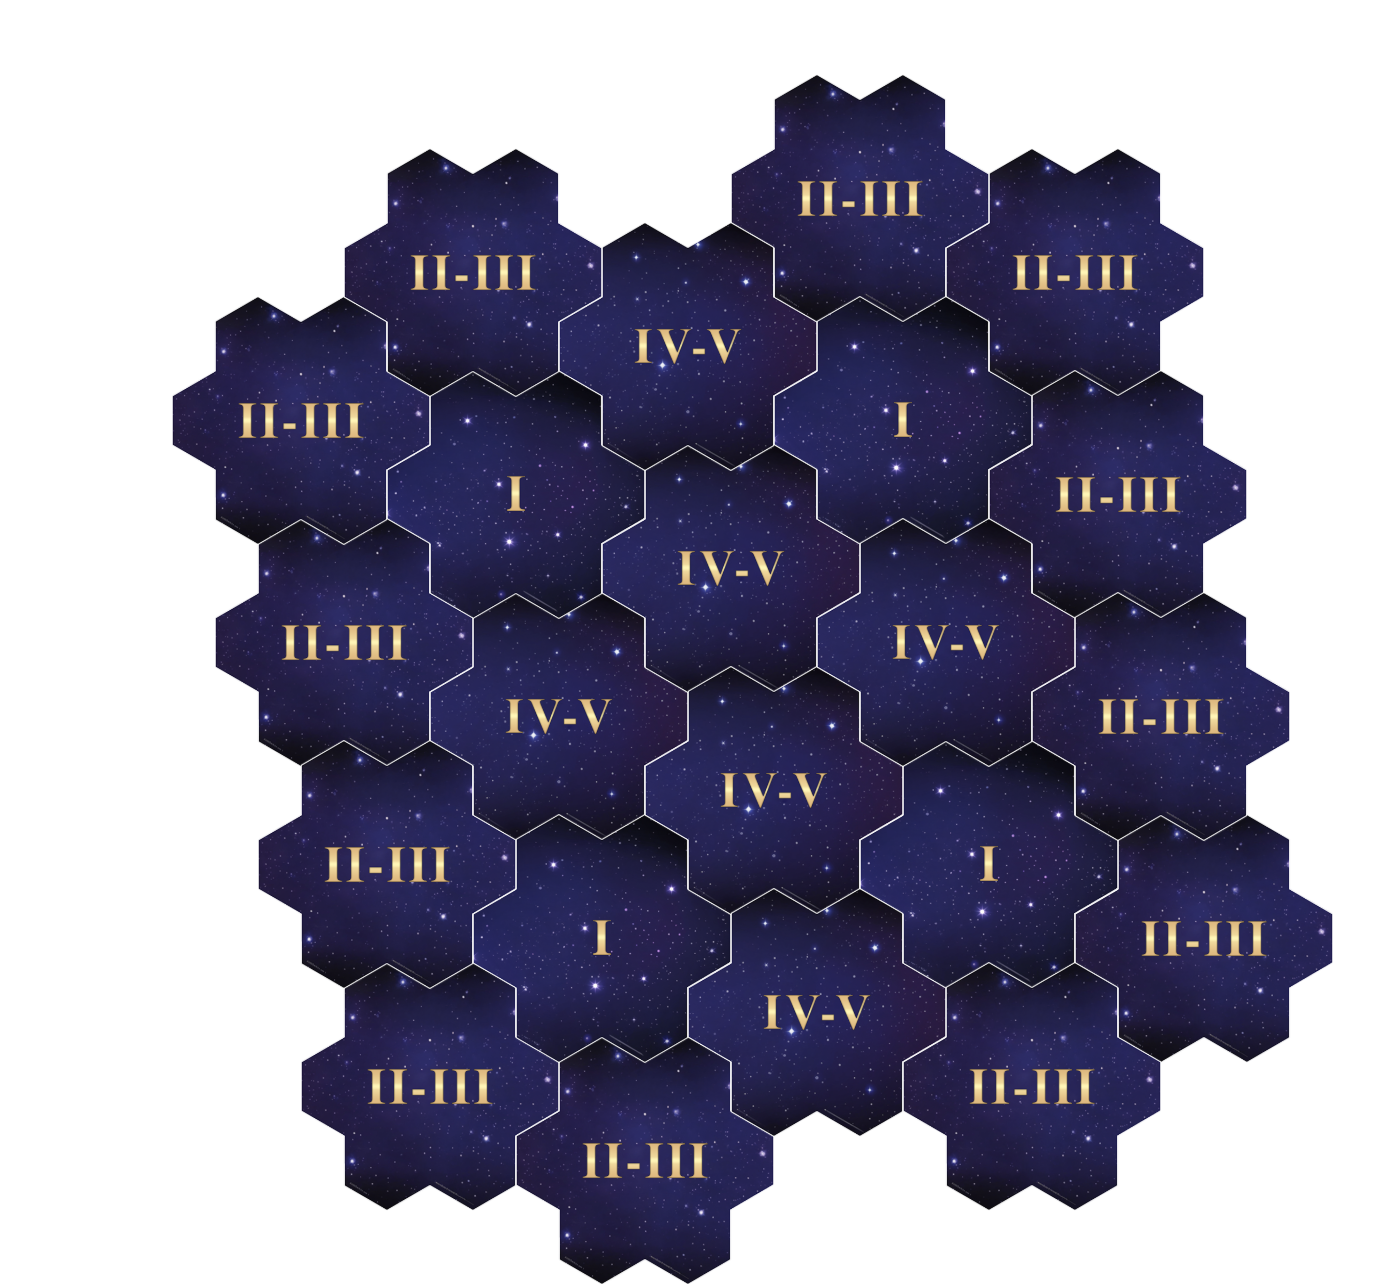
\includegraphics[scale=0.165]{\maps/dragon-valley-4p-short.png}};
  \node at (12.1, -20) {\footnotesize{\textbf{\MakeUppercase{4-PLAYER 8 ROUND SCENARIO}}}};
\end{tikzpicture}
